% \documentclass[fleqn,10pt]{wlscirep}
\documentclass[prx,twocolumn,floatfix,superscriptaddress,longbibliography]{revtex4-1}
\usepackage[utf8]{inputenc}
\usepackage[T1]{fontenc}
\usepackage{bm}
\usepackage{tikz}
\usepackage{subfiles}
\usepackage{mathtools}
\usetikzlibrary{shapes,arrows,positioning}
\usepackage{standalone}
\usepackage{amssymb,amsmath,amstext}
\usepackage{amsthm}
\usepackage{bbm}
\usepackage{graphicx}
\usepackage{epstopdf}
\usepackage{color}
\usepackage{appendix}
\usepackage[T1]{fontenc}
\usepackage{bbold}
\usepackage{bbm}
\usepackage{float}
\usepackage{latexsym}
\usepackage{xr-hyper}
\usepackage[colorlinks=true,citecolor=blue,linkcolor=magenta]{hyperref}
\usetikzlibrary{quantikz2}
\usepackage{braket}
\usepackage{physics}
\usepackage{algpseudocode}
\usepackage{placeins}
\usepackage{multirow}
\usepackage{booktabs}
\graphicspath{{./Figures/}}
%\usepackage[latin1]{inputenc}
%\usepackage{hyphenat}

\usepackage{hhline}
%\bibliographystyle{apsrev4-2}
\def\bibsection{\section{\refname}} 
\usetikzlibrary{shapes,arrows}
\renewcommand{\vec}[1]{\boldsymbol{#1}}  % Bold vectors instead of arrow vectors
%\newcommand{\<}{\langle}
%\renewcommand{\>}{\rangle}

\long\def\ca#1\cb{} %Use for commenting out: \ca...\cb

\def\cites#1{XXX Need citation #1 XX}

\begin{document}

\title{Quantum Algorithms for Portflolio Optimisation and Option pricing}

\author{G. Balarezo}
\thanks{e-mail: juan.balarezo@yachaytech.edu.ec}
\affiliation{School of Physical Sciences and Nanotechnology,\\ Yachay Tech University,\\Urcuqui, Ecuador}


\begin{abstract}
Quantum computing has the promise to address computational problems that are considered intractable with our classical computational models. Nevertheless, due to the current limitations of the available quantum hardware, we are still years away from achieving a universal fault-tolerant quantum computer. In the interim, the development of quantum algorithms for specific problems and their implementation on near-term quantum devices is a promising approach. In this work, we review the most promising quantum algorithms for financial applications, focusing on Portfolio Optimisation and Option Pricing. We describe the ideas behind important quantum algorithms such as Variational Quantum Algorithms (VQAs) and Quantum Amplitude Estimation (QAE) and their theoretical performance. We provide an overview of the hardware available for their implementation and discuss the results 
obtained by some study cases, comparing them with their classical counterparts. Finally, we discuss the future prospects of these algorithms in the financial industry.
  \\
  \textbf{Keywords:} Quantum algorithms, Quantum approximate optimization algorithm, Quantum amplitude estimation, Portfolio optimisation, Quantum computing.
\end{abstract}

\maketitle

\section{Introduction}

Quantum computing has become a rapidly growing field of research in recent years, sparking interest from both academic and industrial sectors, including the financial industry in particular \cite{Hassija2020}. The potential of quantum computers to address computational problems that are considered intractable with our classical models of computation \cite{nielsen2010quantum} has driven a considerable amount of research and innovation in the development of Noisy Intermediate-Scale Quantum computers (NISQ) and quantum algorithms capable of leveraging this computational power \cite{Huang2023}. 

These near-term devices, with limited qubit capabilities and high error rates, have shown promising results. Implemented along with classical computers and adequate quantum algorithms, they can offer significant speedups for some important but classically inefficiently solvable problems in areas such as Optimisation \cite{Symons2023}, Stochastic Modelling \cite{Herbert2022}, and Machine Learning \cite{Zeguendry2023}. These advancements are particularly relevant to the financial sector \cite{Egger2020a}, where they could yield substantial speedups in tasks such as portfolio optimisation and option pricing \cite{Hassija2020}. These tasks have a high 
computational cost that coupled with growing complexity of the financial markets, the need for real-time analysis of large amounts of data and fast decision-making \cite{book:2139036}, makes quantum computing 
an attractive option for financial institutions. 

In the Modern Portfolio Theory (MPT) proposed by Markowistz \cite{Markowitz1952}, the goal of portfolio optimisation is to find the best combination of assets that maximises the return for a given level of risk and some constraints. This is a highly constrained quadratic optimisation problem, known to be NP-Hard, which can be formulated in several ways depending on the conditions of the 
investor \cite{Herman2022}. Machine Learning based models (ML) such as the one proposed by Mazumdar et al. \cite{Mazumdar2020} are widely used for minimising risk contributors and maximising asset diversification.

In particular, quantum approaches to portfolio optimisation are gaining significant attention \cite{Quarterly2020}. In 2019 Kerenidis, Prakash and Szilágyi proposed a quantum algorithm for the constrained portfolio optimisation problem. Based on an interior point method, this algorithm reduces the optimisation problem to a second order cone program (SOCP). The authors suggest that their algorithm could achieve a $\mathcal{O} (n)$ speedup over  its classical counterpart.

Other approaches such as the variational quantum algorithms (VQAs) \cite{Yuan2019, Cerezo2021, McClean2016, Amaro2022} work by reformulating the portfolio optimisation problem as a 
quadratic unconstrained binary optimisation (QUBO) problem. Glover et al. \cite{Glover2019} covers some methods to reformulate any optimisation problem as a QUBO problem, and Date et al. \cite{Date2019} proposed an algorithm that allows the efficient embedding of a QUBO problem in a quantum annealer.  Using these concepts, Variational Quantum 
Eigensolver (VQE) \cite{Huang2023, McClean2016, Peruzzo2014, Barkoutsos2020, Buonaiuto2023} and Quantum Approximate Optimisation Algorithm (QAOA) \cite{Farhi2014, Blekos2024} have been proposed for portfolio optimisation \cite{Egger2020}. Quantum annealers such as those developed by D-Wave Systems \cite{King2023} are been used for practical implementations of the aforementioned algorithms
\cite{Yarkoni2022, Phillipson2020, Venturelli2019}. Nevertheless, it remains unclear whether these quantum algorithms provide any effective speedup over classical methods for these tasks.

Option pricing is another important task in finance where quantum algorithms have been applied. The implementation of the
Quantum Amplitude Estimation (QAE) algorithm \cite{Woerner2019, Nakaji2020, Stamatopoulos2020, Rebentrost2018} has been proposed for the calculation of the expected value of the option price. This algorithm is

\begin{table*}[t!] 
  \begin{center}
    \caption{\label{Tab:paper_overview} Criteria for the selection of the papers reviewed in this work.}
    \begin{tabular}{c|c|c|c} \hline \hline
\textbf{Metodology} &
  \textbf{Application} &
  \textbf{Algorithm} &
  \textbf{Hardware} \\ \hline
Optimisation &
  \begin{tabular}[c]{@{}c@{}}Portfolio \\ optimisation\end{tabular} &
    \begin{tabular}[c]{@{}c@{}}Approximate \\ Optimisation\\ (SOCP, VQE, QAOA) \\
    \cite{Mazumdar2020}, \cite{Buonaiuto2023}, \cite{Phillipson2020}, \cite{Venturelli2019}  \end{tabular} &
  \begin{tabular}[c]{@{}c@{}}Gate-based quantum computer \\ Quantum Annealer\end{tabular} \\ \hline  
    %\multicolumn{1}{}{  Gate-based quantum computer \\ Quantum Annealer} \\ \hline
Monte Carlo &
  \multicolumn{1}{l|}{\begin{tabular}[c]{@{}l@{}}Option pricing \end{tabular}} &
  \begin{tabular}[c]{@{}c@{}}Search and Count\\ (QAE, QPA, QPE) \\ 
  \cite{Woerner2019},\cite{Nakaji2020}, \cite{Stamatopoulos2020}, \cite{Rebentrost2018}, \cite{Rebentrost2022} \end{tabular} &
\begin{tabular}[c]{@{}c@{}} Gate-based quantum \\ computer\end{tabular} \\ \hline \hline
\end{tabular}
\end{center}
\end{table*}

expected to provide a quadratic speedup over the classical Monte Carlo methods used for this task. 

The aim of this work is to provide a review of the quantum algorithms for specific financial applications, focusing on Portfolio Optimisation and Option Pricing. Table \ref{Tab:paper_overview} provides an overview of the topics covered in this work, as well as the relevant literature reviewed. 

In Sec. \ref{sec:background} we introduce necessary concepts in finance and quantum algorithms. Then, in Sec. \ref{sec:literature1} and Sec. \ref{sec:literature2}  we present a review of relevant literature on quantum algorithms proposed for the aforementioned financial applications. We also 
  introduce the classical methods used for these tasks and compare them with their quantum counterparts.

In Sec. \ref{sec:hardware} we provide an overview of the hardware implementations of these algorithms. Finally, Sec. \ref{sec:discussion} concludes this work and discusses the future prospects of quantum algorithms in the financial industry. 

It is worth mentioning that important surveys have been published on the topic of quantum computing in finance in recent years. Among these, we highlight the works of Orús et al. \cite{Orus2019}, Egger et al. \cite{Egger2020a}, Albareti et al. \cite{Albareti2022}, Herman et al. \cite{Herman2022}, and Herman et al. \cite{Herman2023}, which have been instrumental in the development of this work. We refer the interested readers to these works for a more comprehensive overview of the field.

\section{background}\label{sec:background}
\subsection{Some basics concepts}
\subsubsection{Assets and Portfolio Optimisation}

In finance, an asset is a financial instrument that can be owned by an individual, a corporation, or a country with the expectation that it will provide a future benefit \cite{2023}. Financial assets can include stocks, bonds, commodities, derivatives, etc. 

On the other hand, a portfolio is a set of individual investments that may include a wide range of asset classes. A portfolio is characterised by components such as diversification, risk and return, and asset allocation. The main goal of a portfolio is to diversify investments to achieve some specific objective such as maximising returns, minimising risk, or a balance between them \cite{Wilmott2007}. 
In order to achieve this, portfolio optimisation is used to find the best allocation of assets that fulfils the investor's objectives.

In the original work by Markowitz \cite{Markowitz1952}, a mean-variance portfolio optimisation (MVPO) is proposed, which is widely used used in the financial industry to this day, and whose formulation is presented in this section.

The input for the MVPO is the historical prices and returns of the considered financial assets. An asset range $(1 \leq i \leq N)$ is considered, and a time range $(0 \leq t \leq T)$. 

Then, the first step is to obtain a list $P$ of current prices $P_i$  of the assets of interest.
\begin{equation}
  \label{eq:1}
  P_i = p_i(T)
\end{equation}

In addition, the historical returns of the assets between time $t-1$ and $t$ are calculated as:
\begin{equation}
  \label{eq:2}
  r_i(t) = \frac{p_i(t) - p_i(t-1)}{p_i(t-1)}
\end{equation}

But for inference purposes, we must consider the expected return of the assets. So, given the historical returns, we can calculate the expected return of the assets as:
\begin{equation}
  \label{eq:3}
  \mu_i = \frac{1}{T} \sum_{t=1}^{T} r_i(t)
\end{equation}

The variance of the returns of each asset and the covariance between returns of different assets over the historical period are given by:
\begin{equation}
  \label{eq:4}
  \sigma_i^2 = \frac{1}{T-1} \sum_{t=1}^{T} (r_i(t) - \mu_i)^2
\end{equation}
\begin{equation}
  \label{eq:5}
  \sigma_{ij} = \frac{1}{T-1} \sum_{t=1}^{T} (r_i(t) - \mu_i)(r_j(t) - \mu_j)
\end{equation}

A set of investments $x_i$ (given as a fraction of the total budget or number of asset units) allocated for each $i$th considered asset, 
is then defined. Therefore, an optimal method for asset allocation aims to maximise the portfolio return 
$\mu^\text{T} x$ while minimising risk, defined as the portfolio variance $x^\text{T}\Sigma x$, where $\mu$ is the vector of expected returns for each asset $i$ computed by Eq. \ref{eq:3}, $\Sigma$ is the covariance matrix calculate by Eq. \ref{eq:4} and Eq. \ref{eq:5}, and $x$ is the vector 
of asset allocations measured as fractions of the total budget. Therefore, the problem of finding the optimal portfolio is reduced to find the $x$ vector that maximises the following objective function: 
\begin{equation}
  \label{eq:6}
  \mathcal{L}(x) = \mu^\text{T} x - q x^\text{T}\Sigma x
\end{equation}
where $q$ is a parameter that determines the trade-off between risk and return.  In a realistic scenario, budget constraints and non-negative 
$x_i$ values (only buying) must be considered. Therefore, in the general case, the problem is formulated as follows:
\begin{equation}
\begin{aligned}
  \label{eq:7}
  \max_{x} \mathcal{L}(x): & \max_{x}\left(\mu^\text{T} x - q x^\text{T}\Sigma x \right) \\ 
  \text{s.t.} & \quad \sum_{i=1}^{N} x_i = 1 
\end{aligned}
\end{equation}
In section \ref{sec:literature1} we will review how this problem can be mapped into a QUBO problem and solved using quantum algorithms.

\subsubsection{Option Pricing}
An option is a financial instrument that gives the holder the opportunity but not the obligation to buy or sell the  \textbf{underlying asset} at an agreed-upon price (\textbf{strike price}) at a specified time in the future (\textbf{expiration date}) \cite{Wilmott2007}. There are many kind of options, 
but the most common are \textbf{call} and \textbf{put options} (buy and sell options, respectively). Furthermore, we must 
differentiate between European and American options. The former can only be exercised at the expiration date, while the latter can be exercised at any time before the expiration date \cite{Rebentrost2018}. 
\begin{figure}
\centering
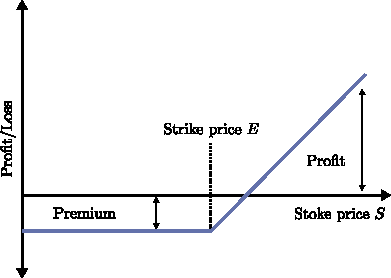
\includegraphics[width=0.45\textwidth]{pay-off.pdf}
  \caption{\label{fig:profit-diagram} Profit diagram for a call option. Adapted from \cite{Wilmott2007}.}
\end{figure}

The profit diagram for a call option is shown in Fig. \ref{fig:profit-diagram}, where the \textbf{premium} is the price paid for contract initially. Then, the 
intrinsic value of the option at the expiration date is calculated as the difference between the stock price $S$ and the strike price $E$. 
This function of the underlying asset is called the \textbf{payoff function} and is given by:
\begin{equation}
  \label{eq:8}
  \text{Payoff} = \max(S - E, 0)
\end{equation}

The purpose of option pricing is to estimate Eq. \ref{eq:8} at the expiration date and then, determine the \textbf{fair value}, which indicates the amount of money an 
investor should pay to enter the option contract today, given the current market conditions. 
The challenging part is to compute the expected value of the option payoff, which is usually done using Monte Carlo methods. In section \ref{sec:literature2} we will discuss the quantum approach to 
this problem.

\subsection{Variational Quantum Algorithms}
Variational Quantum Algorithms (VQAs) are hybrid quantum-classical algorithms that 
are well suited for NISQ devices and allow us to get approximate solutions to optimisation and combinatorial problems efficiently \cite{Cerezo2021}. This algorithms rely on the fact that we can, in 
principle, reformulate any optimisation problem as a QUBO problem \cite{Glover2019}.  

QUBO problems can not directly be cast into a quantum computer, but they share a isomorphism with the Ising Hamiltonian, making it easy to map a QUBO problem into an Ising Hamiltonian, which can be cast into adequate quantum operators in a quantum computer \cite{Buonaiuto2023}. 
\begin{figure}[h!]
\centering 
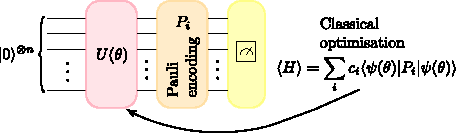
\includegraphics[width=0.5\textwidth]{VQE-Buonaiuto.pdf}
  \caption{\label{fig:vqe} Variational Quantum Eigensolver (VQE) algorithm. Adapted from \cite{Buonaiuto2023}.}
\end{figure}

One of the VQAs used for portfolio optimisation is the Variational Quantum Eigensolver (VQE) algorithm (see Fig. \ref{fig:vqe}). The aim of the VQE algorithm is to find an approximate value for the ground state energy of a given Hamiltonian.  

The starting point is to define a cost function
\begin{equation}
  \label{eq:9}
  C(\boldsymbol{\theta}) =\langle\psi(\boldsymbol{\theta})|H|\psi(\boldsymbol{\theta})\rangle
\end{equation}
where $H$ is the Hamiltonian of our problem, that can be written as the weighted sum of Pauli operators \cite{Tilly2022}, such
\begin{figure*}[ht!]
  \begin{center} 
  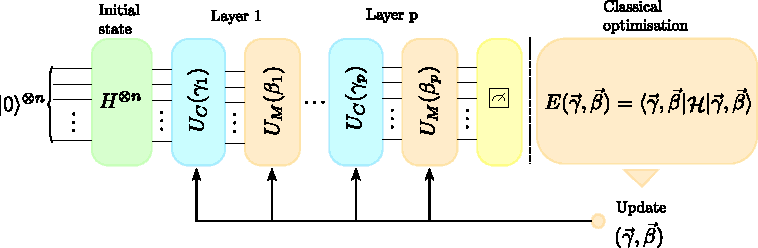
\includegraphics[width=0.85\textwidth]{QAOA-Blekos.pdf}
  \caption{\label{fig:qaoa} Quantum Approximate Optimisation Algorithm (QAOA). Adapted from \cite{Blekos2024}.}
  \end{center}
\end{figure*}
that: 
\begin{equation}
  \label{eq:10}
  \mathcal{H} = \sum_{i} c_i P_i
\end{equation}
where $P_i \in \{I, X, Y, Z\}^{\otimes N}$ are called Pauli strings and $N$ is the number of qubits, and $c_i$ are the coefficients of the Pauli strings.  Additionally, $\boldsymbol{\theta}$ is a set of trainable parameters for some trial state $|\psi(\boldsymbol{\theta})\rangle = U(\boldsymbol{\theta}) |0\rangle ^{\otimes n}$. So, Eq. \ref{eq:9} becomes:
\begin{equation}
  \label{eq:11}
  C(\boldsymbol{\theta}) =\sum_i c_i \langle \boldsymbol{0}|U(\boldsymbol{\theta})^\dagger P_i U(\boldsymbol{\theta})|\boldsymbol{0}\rangle
\end{equation}
for some ansatz $U(\boldsymbol{\theta})$, that can be written as
\begin{equation}
  \label{eq:12}
  U(\boldsymbol{\theta}) = \prod_{k=1}^{p} e^{-i\theta_k \mathcal{H}_k}
\end{equation}
where $\mathcal{H}_k$ are the terms of the Hamiltonian $\mathcal{H}$  and $p$ determines the precision of the approximation \cite{Cerezo2021}.

Therefore, the VQE consists of classical algorithm that uses a quantum algorithm as a subroutine. We first initialise the state 
$|\psi(\boldsymbol{\theta})\rangle$ with some initial parameters $\boldsymbol{\theta}$, then we measure Eq. \ref{eq:11} and use a classical optimisation algorithm to update 
the parameters $\boldsymbol{\theta}$ until we reach a minimum value of $C(\boldsymbol{\theta})$.

The variational principle ensures that at some point the VQE algorithm will converge to:
\begin{equation}
  \label{eq:13}
  E_0 \leq \frac{\langle \psi(\boldsymbol{\theta})|\mathcal{H}|\psi(\boldsymbol{\theta})\rangle}{\langle \psi(\boldsymbol{\theta})|\psi(\boldsymbol{\theta})\rangle}
\end{equation}
where $E_0$ is the ground state energy of the Hamiltonian $\mathcal{H}$ and $|\psi(\boldsymbol{\theta})\rangle$ is some trial state.

In a similar fashion, the Quantum Approximate Optimisation Algorithm (QAOA) is another VQA that was first 
conceived as 


\subsubsection{Quantum Amplitude Estimation}


\section{Portfolio Optimisation}\label{sec:literature1}



\subsection{Classical Portfolio Optimisation}

\subsection{Quantum Portfolio Optimisation}


\section{Option Pricing}\label{sec:literature2}

\subsection{Classical Option Pricing}

\subsection{Quantum Option Pricing}


\section{Hardware Implementations}\label{sec:hardware}




\section{Discussion and Conclusion}\label{sec:discussion}



\FloatBarrier

\bibliography{/home/pacman/Documents/git-repositories/quantum-computing/lecture-notes/bibliography.bib}

\end{document} 
